\subsection{Diseño Arquitectónico y Acondicionamiento del VCO-RF}
La síntesis de un oscilador controlado por tensión (VCO) en radiofrecuencia con entradas de magnitud y frecuencia instantánea requiere una etapa de acondicionamiento de fase previa[cite: 308]. Dado que la oscilación se rige por la acumulación angular $\theta(t) = 2\pi \int f(t) dt$, se intercepta la señal de frecuencia ($f_{in}$) antes del oscilador base. 

Para traducir el parámetro de desviación en Hertz ($f_d$) a radianes por muestra, se deduce el factor de escalado basado en el periodo de muestreo ($T_s = 1/f_s$) y la frecuencia angular deseada ($\omega_d = 2\pi f_d$):
\begin{equation}
    \Delta\theta = 2\pi f_d \cdot \frac{1}{f_s} = \frac{2\pi f_d}{f_s}
    \label{eq:escalado}
\end{equation}

Este valor constituye la constante del bloque \texttt{Multiply Const}, la cual alimenta a un integrador discreto (\texttt{e\_Acum}) para generar la rampa de fase continua inyectada al puerto \texttt{in 1} del VCO subyacente.

El diseño propuesto se evidencia en el diagrama de bloques de la Figura \ref{fig:diagrama_vco}, el cual encapsula la conversión matemática para lograr un control lineal de la frecuencia[cite: 15, 313].

\begin{figure}[H]
    \centering
    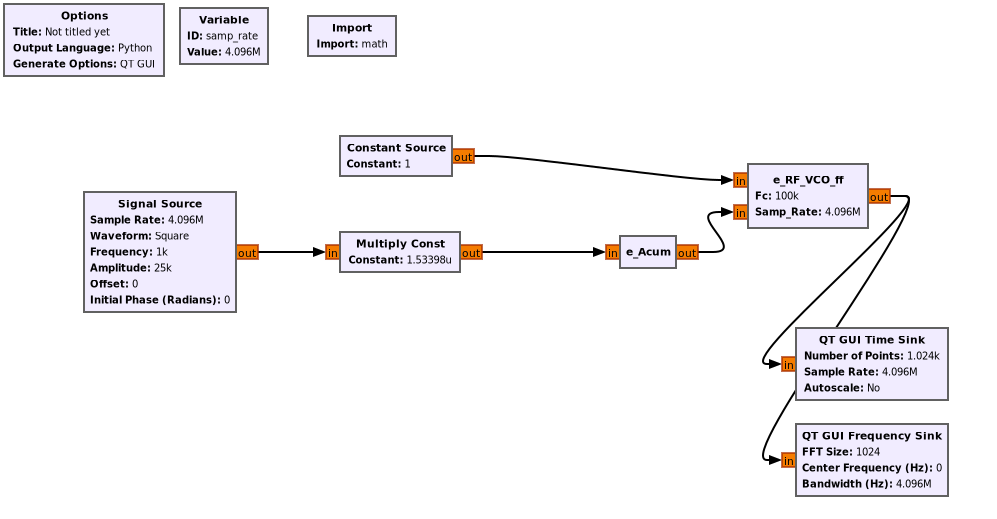
\includegraphics[width=0.95\linewidth]{imagenes/propuesta.png}
    \caption{Diagrama de bloques del subsistema VCO-RF diseñado.}
    \label{fig:diagrama_vco}
\end{figure}